\subsection{Постановка задачи разработки системы индексации блокчейн данных}

На основании анализа предметной области задача настоящей выпускной
квалификационной работы заключается в разработке системы индексации
блокчейн данных сети Bitcoin, обеспечивающей получение информации от доверенного узла,
ее нормализацию, транзакционное сохранение в реляционной базе данных и
предоставление внешним потребителям через прикладной интерфейс.

Разрабатываемая система должна решать следующие основные задачи:
\begin{enumerate}
    \item выполнять последовательную индексацию блоков и транзакций канонической цепи;
    \item формировать и поддерживать актуальный набор \gls{utxo}, адресные балансы
    и их исторические представления;
    \item обрабатывать изменения состояния mempool и учитывать reorg заданной глубины;
    \item предоставлять \gls{api} для управления заданиями индексирования и выдачи данных;
    \item обеспечивать наблюдаемость, управляемость и пригодность к контейнерному развертыванию.
\end{enumerate}

Для формализации потоков данных используется нотация DFD. Она позволяет
последовательно перейти от внешних границ системы к внутренним процессам,
хранилищам и специализированным сценариям обработки. В рамках постановки
задачи применена многоуровневая декомпозиция: контекстная диаграмма фиксирует
границы ответственности, на диаграмме первого уровня раскрываются основные
процессы, а на диаграммах второго уровня детализируются критические процессы
индексации, администрирования заданий и выдачи данных.

Границы проектируемой системы и ее место в общей инфраструктуре показаны на
рисунке~\ref{fig:context-dfd}. Из диаграммы следует, что индексер выступает
промежуточным звеном между узлом Bitcoin, административными и пользовательскими
клиентами, а также подсистемой хранения данных.

\begin{figure}
  \centering
  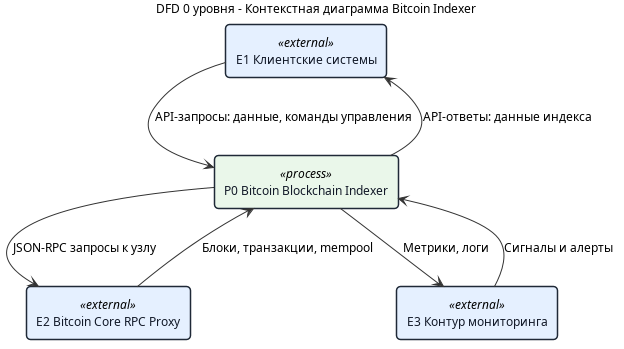
\includegraphics[width=0.9\linewidth]{../report/dfd/DFD_Level_0_Context.png}
  \caption{Контекстная DFD-диаграмма системы индексации блокчейн данных}
  \label{fig:context-dfd}
\end{figure}

Контекстная диаграмма фиксирует внешнюю границу ответственности системы. Узел
Bitcoin Core рассматривается как источник первичных блокчейн данных, PostgreSQL
--- как внешнее состояние stateless-приложения, а административной панели, CLI
и внешним клиентам доступ к индексатору предоставляется только через прикладные
интерфейсы. Такое разбиение соответствует выбранному архитектурному подходу:
серверное приложение не хранит критическое состояние локально и может быть
повторно запущено без потери прогресса индексации.

Декомпозиция контекстного процесса представлена на рисунке~\ref{fig:dfd-level-1}.
На данном уровне система разделяется на три функциональных процесса:
индексацию данных, администрирование заданий и получение/выдачу данных.
Операционное хранилище индексера отделено от хранилища конфигурации и
состояния jobs, поскольку для этих групп данных характерны разные роли в
жизненном цикле системы: первая группа отражает индексированные
блокчейн-сущности, а вторая фиксирует управляющее состояние обработки.

\begin{figure}
  \centering
  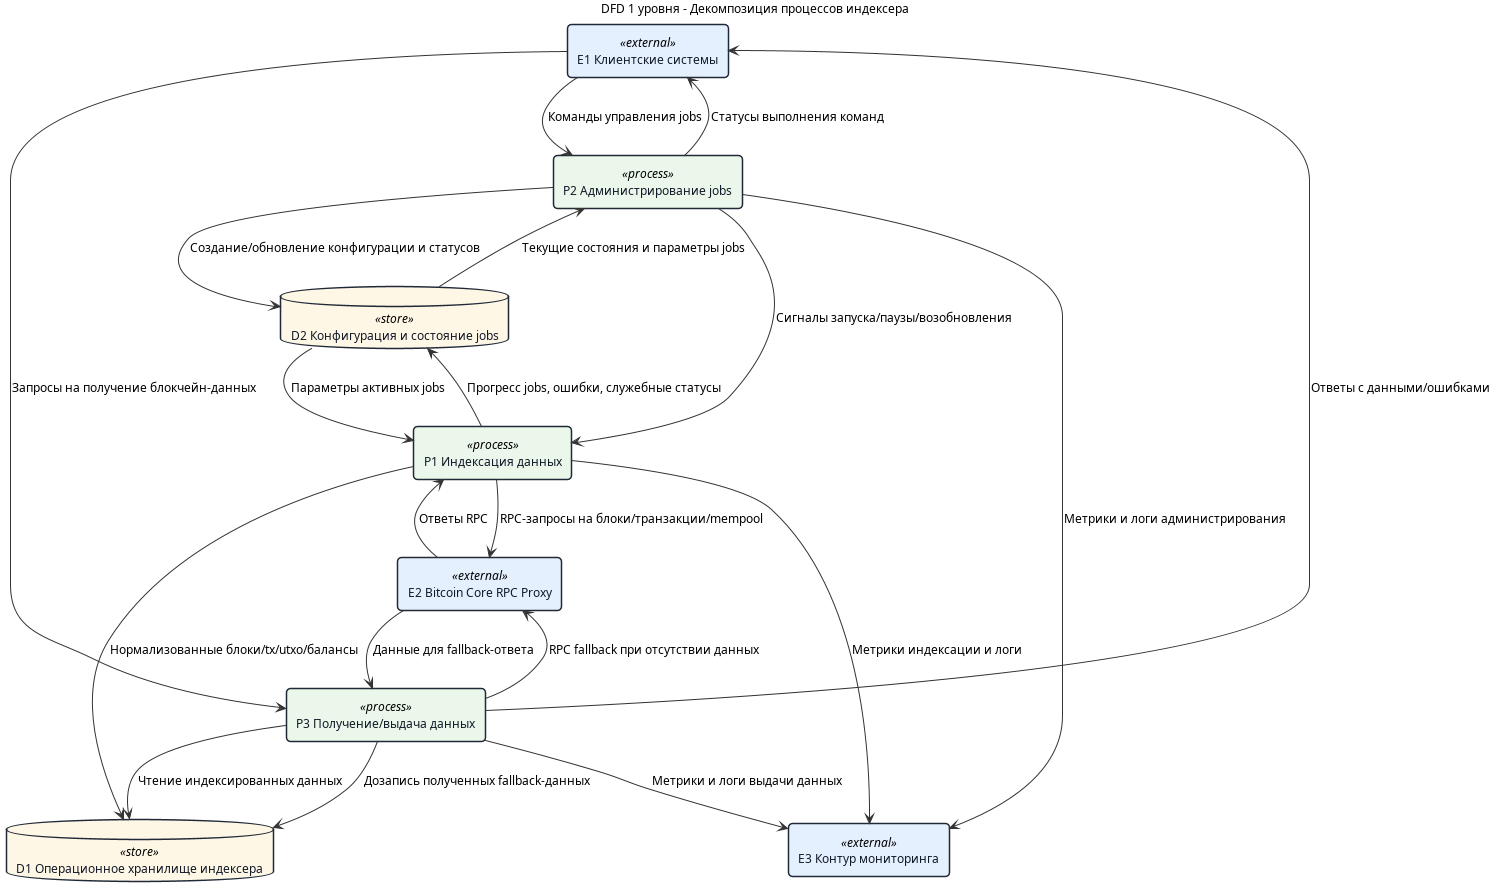
\includegraphics[width=\linewidth,height=0.72\textheight,keepaspectratio]{../report/dfd/DFD_Level_1.png}
  \caption{DFD-диаграмма первого уровня: декомпозиция процессов индексера}
  \label{fig:dfd-level-1}
\end{figure}

На диаграмме первого уровня показано, что между процессом администрирования
jobs и процессом индексации передаются только управляющие сигналы, тогда как
запись нормализованных блоков, транзакций, UTXO и балансов выполняется через
операционное хранилище. Подготовленные представления считываются из индекса, а
при необходимости допускается обращение к RPC proxy как к резервному источнику.
Такое разделение снижает связанность между контуром
управления, контуром фоновой обработки и контуром пользовательских запросов.

Критический поток подтвержденной индексации детализирован на
рисунке~\ref{fig:dfd-level-2-indexing}. Он начинается с определения tip цепи и
диапазона синхронизации, после чего выполняется загрузка блоков и транзакций,
проверка reorg, нормализация данных и фиксация прогресса задания.

\begin{figure}
  \centering
  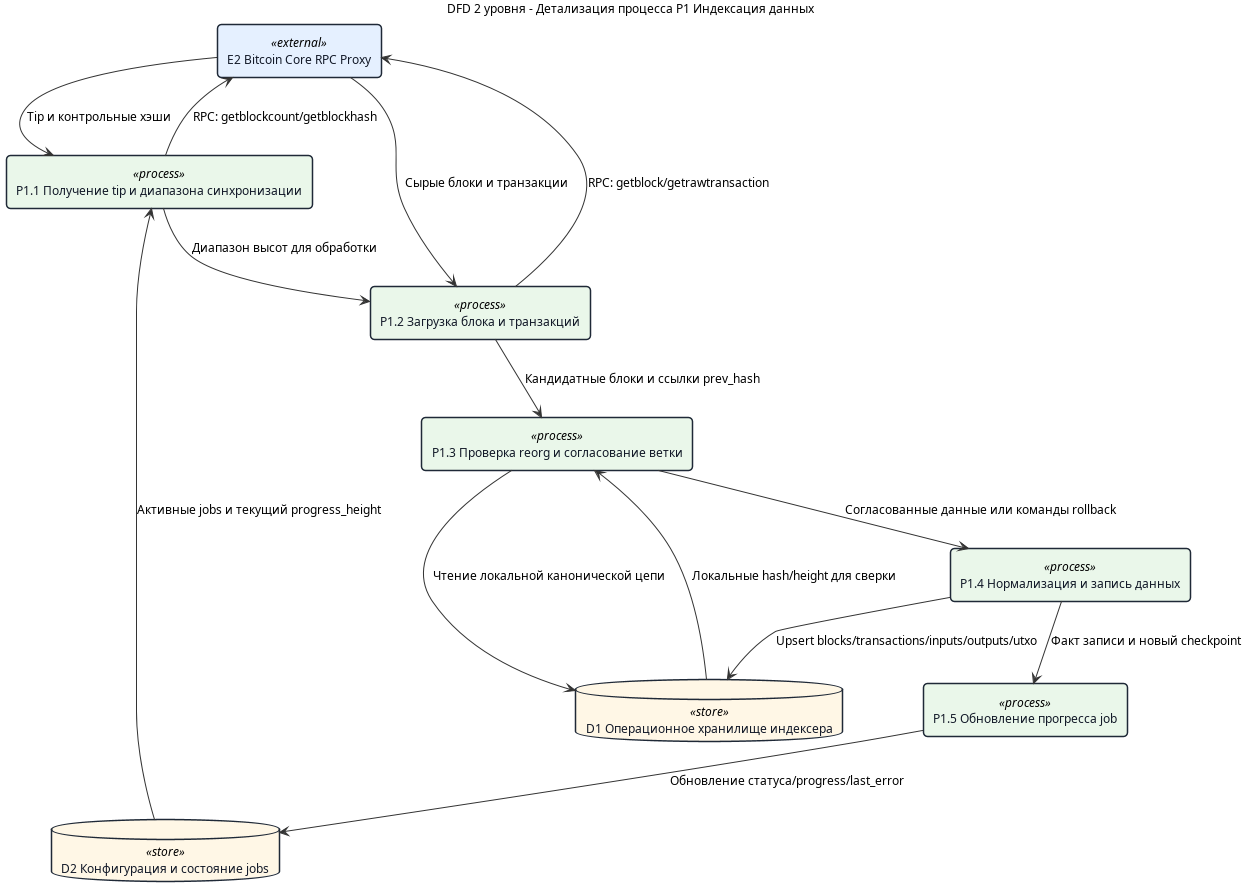
\includegraphics[width=\linewidth,height=0.72\textheight,keepaspectratio]{../report/dfd/DFD_Level_2_Indexing.png}
  \caption{DFD-диаграмма второго уровня: детализация процесса индексации данных}
  \label{fig:dfd-level-2-indexing}
\end{figure}

Декомпозиция индексации подчеркивает, что проверка согласованности цепи
выделяется в самостоятельный процесс между загрузкой блока и записью данных.
Это важно для предметной области Bitcoin: новый блок не может быть
рассмотрен изолированно, так как его связь с предыдущим хэшем определяет
принадлежность к канонической ветке. Поэтому запись в PostgreSQL выполняется
после сверки локального состояния и только затем обновляется прогресс job.

Контур управления заданиями индексирования представлен на
рисунке~\ref{fig:dfd-level-2-admin}. Он описывает обработку команд
создания, запуска, приостановки, возобновления и остановки job.

\begin{figure}
  \centering
  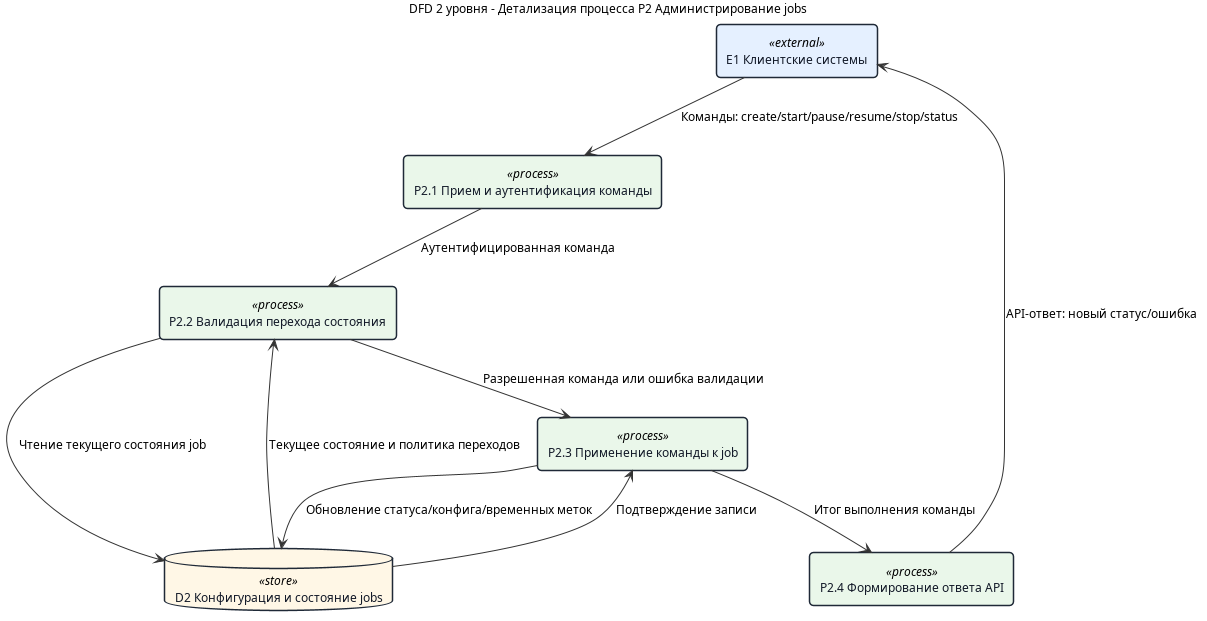
\includegraphics[width=\linewidth,height=0.68\textheight,keepaspectratio]{../report/dfd/DFD_Level_2_Admin.png}
  \caption{DFD-диаграмма второго уровня: детализация процесса администрирования jobs}
  \label{fig:dfd-level-2-admin}
\end{figure}

На этом уровне явно фиксируется, что изменение состояния задания не выполняется
непосредственно после получения команды. Сначала команда проходит
аутентификацию и валидацию допустимого перехода состояния, затем применяется к
записи job и только после этого преобразуется в API-ответ. Такое описание
обосновывает необходимость формализованного жизненного цикла задания и
согласуется с последующим описанием модуля \texttt{jobs}.

Процесс получения и выдачи данных раскрыт на
рисунке~\ref{fig:dfd-level-2-data-serving}. Диаграмма показывает обработку
прикладных запросов к блокам, транзакциям, адресам и mempool.

\begin{figure}
  \centering
  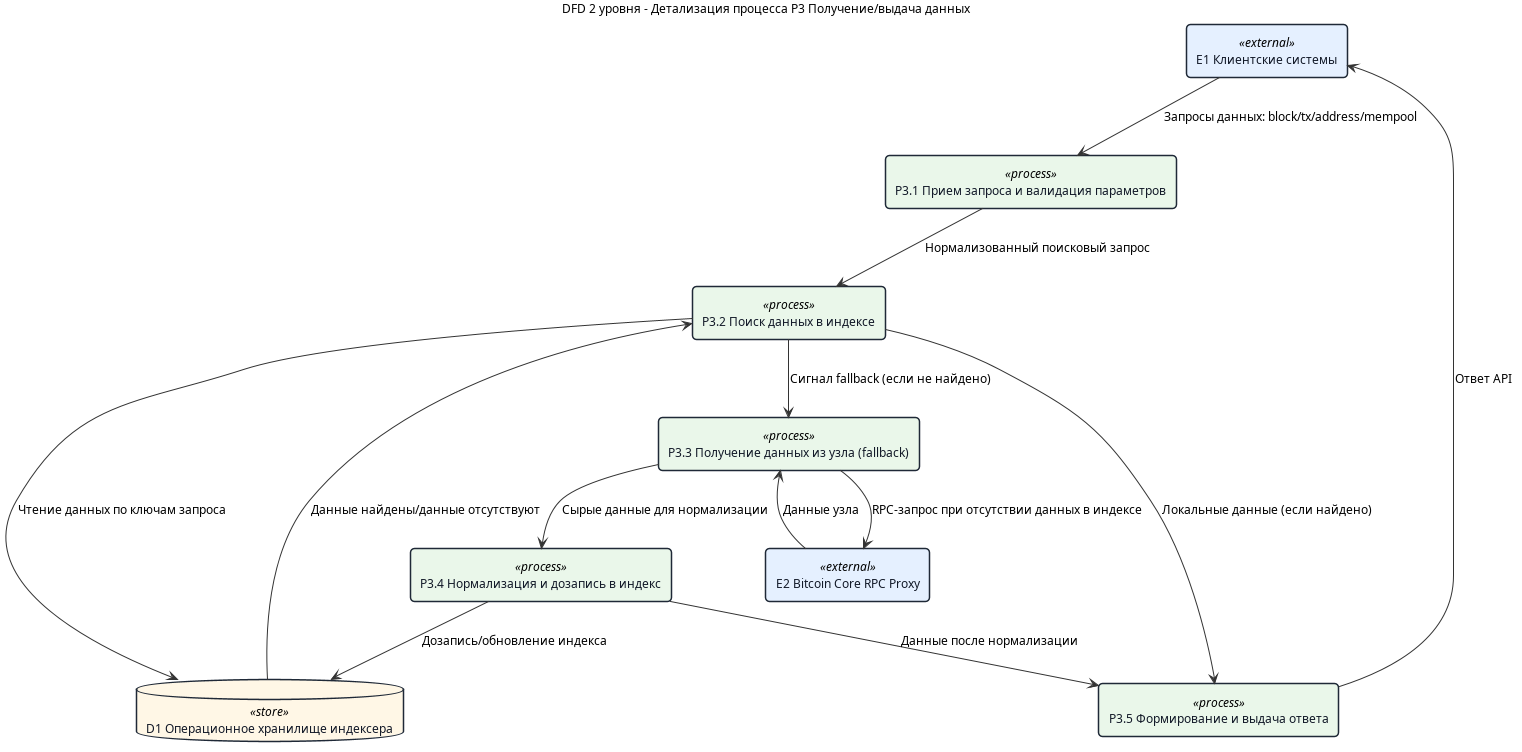
\includegraphics[width=\linewidth,height=0.72\textheight,keepaspectratio]{../report/dfd/DFD_Level_2_DataServing.png}
  \caption{DFD-диаграмма второго уровня: детализация процесса получения и выдачи данных}
  \label{fig:dfd-level-2-data-serving}
\end{figure}

Для контура выдачи данных принципиально важно разделение поиска в локальном
индексе и резервного обращения к узлу. При наличии данных ответ формируется на
основе подготовленных представлений PostgreSQL. Если данных в индексе нет,
допускается обращение к Bitcoin Core RPC proxy с последующей нормализацией и
дозаписью результата. В результате для внешнего клиента сохраняется единый API-контракт,
а внутренняя система сохраняет возможность постепенно пополнять индекс без
нарушения границ stateless backend-приложения.

С учетом особенностей предметной области итоговая постановка задачи сводится
к созданию программной системы Bitcoin Blockchain Indexer,
обеспечивающей устойчивую, управляемую и воспроизводимую индексацию
блокчейн данных сети Bitcoin, достаточную для использования в прикладных,
аналитических и исследовательских сервисах. Тем самым в работе решается
задача построения промежуточного инфраструктурного слоя между узлом Bitcoin и
внешними потребителями данных.
